\documentclass[11pt,a4paper]{article}

% ---------- Packages ----------
\usepackage[left=1.5in,right=1in,top=1in,bottom=1in]{geometry}
\usepackage{tikz}
\usetikzlibrary{arrows.meta,positioning,shapes.geometric,calc}
\usepackage{booktabs}
\usepackage{cite}
\usepackage{amsmath,amssymb}
\usepackage{xcolor}
\usepackage{enumitem}
\usepackage{parskip}

\definecolor{tocblue}{RGB}{22,42,110}

\usepackage[colorlinks=true,linkcolor=tocblue,citecolor=tocblue,urlcolor=tocblue]{hyperref}

\setlength{\parskip}{0.5em}
\setlength{\parindent}{0pt}
\linespread{1.0}

\title{The Speculation Tax}
\author{[Your Name], Entry No.\ [Entry Number] \\{} [Partner Name], Entry No.\ [Entry Number]}
\date{24 August 2026}

\hypersetup{
  pdftitle={The Speculation Tax: A Security-Performance Study of Cache-Timing Side Channels and Their Hardware Mitigations},
  pdfauthor={ELL305 Term Paper Group}
}

\begin{document}

% ------------------------------------------------------------
% Paste this block immediately AFTER \maketitle (or \begin{document}
% if no titlepage macro is used) and BEFORE \tableofcontents.
% Requires no extra packages beyond a standard article/report class;
% if using a class without an `abstract` environment, wrap the
% same content in an `abstract` minipage or the class's preferred
% \begin{abstract}...\end{abstract} substitute.
% ------------------------------------------------------------


% ---------- Title Page ----------
\begin{titlepage}
\centering
\vspace*{3.2cm}
{\Huge\bfseries The Speculation Tax\par}
\vspace{0.5cm}
{\Large\bfseries A Security--Performance Study of Cache-Timing\\ Side Channels and Their Hardware Mitigations\par}
\vspace{1cm}
{\normalsize\itshape Working title: Microarchitectural Security --- The True Cost of\\ Mitigation and Whether Speculation Can Be Made Safe\par}

\vspace{2.2cm}
{\large ELL305 Term Paper\par}
\vspace{0.3cm}
{\large Akshat Pandey, 2024EE10785\par}
{\large Anirudh K. Garg, 2024EE11066\par}
{\large Dravya Mehta, 2024EE11099\par}
{\large Ujjawal Mishra, 2024EE10745\par}
{\large Uplaksh Bishnoi, 2024EE11162\par}
{\large Viradiya Darsh, 2024EE10514\par}

\vfill

{\large ELL305 \quad Draft \#1 (progress report)\par}
\vspace{0.2cm}
{\large Draft \#1 due 24 August 2026 \quad$\vert$\quad Final due 11 November 2026\par}
\vspace{2.5cm}
\end{titlepage}

% ---------- Table of Contents ----------
\clearpage
\tableofcontents
\clearpage

\section*{\Huge{Abstract}}
Modern out-of-order processors sustain high throughput via speculative execution. While branch mispredictions trigger precise architectural rollbacks, they leave persistent microarchitectural footprints in the cache hierarchy. Attackers exploit this asymmetry using timing channels (e.g., Flush+Reload) to extract secret data, as demonstrated by the Spectre and Meltdown vulnerabilities. This progress report investigates whether speculative execution can be secured without fundamentally crippling processor performance. We categorize current hardware mitigations into a four-strategy taxonomy—fencing, invisible speculation, cache partitioning, and taint tracking—and outline a two-pronged evaluation methodology. First, we conduct empirical covert-channel bandwidth measurements on commodity x86 hardware to calibrate cache-timing latencies. Second, we utilize a cycle-level architectural simulation platform to quantify the Instructions Per Cycle (IPC) degradation imposed by strict speculation constraints across various benchmark classes. Ultimately, by synthesizing these empirical and simulated metrics, our final paper will construct a quantitative security-performance Pareto curve to evaluate why perfectly secure architectures remain impractical under modern power-performance-area (PPA) constraints.
\clearpage

% \noindent\textbf{Keywords:} speculative execution; transient execution attacks; microarchitectural side channels; cache-timing covert channels; Flush+Reload; Prime+Probe; Spectre; Meltdown; Foreshadow; out-of-order execution; reorder buffer; hardware security mitigations; invisible speculation; cache partitioning; speculative taint tracking; IPC overhead; power-performance-area (PPA) trade-offs; architectural simulation

% ------------------------------------------------------------
% End of abstract block.
% ------------------------------------------------------------
\section{Work Done as of 24 August 2026}

\subsection{Chosen Topic}
This document is a \emph{progress report} (Draft~\#1), not a finished paper: it
records the work completed as of 24 August 2026 and states the plan for the
remaining work packages, so every claim it makes about experiments is a
statement of intent rather than a result. In keeping with the guidance we have
received on scoping and supervision, I will consult \textbf{Prof.\ Sumantra DuttaRoy} as
ADVISED.



Our term paper studies microarchitectural security, and specifically the family of
vulnerabilities known as \emph{transient-execution attacks}. Modern high-performance
processors are, almost without exception, deeply speculative machines: they predict
branch outcomes, prefetch data, reorder memory operations, and execute instructions
before it is known whether those instructions should architecturally execute at all.
Speculation is not an optional performance trick but a load-bearing part of how a
modern out-of-order core sustains high instruction throughput in the presence of
multi-hundred-cycle memory latencies. Our paper studies the security consequence of
this design choice: speculatively executed instructions, even when their results are
eventually squashed and never committed to architectural state, leave measurable
side effects in microarchitectural structures --- most importantly the cache hierarchy.
An attacker who can measure those side effects, typically through cache-timing
channels such as Flush+Reload or Prime+Probe, can recover data that was never
supposed to be architecturally visible to them.

The \textbf{scope of the paper} is deliberately bounded to keep the investigation tractable
within the term. We cover (i) the microarchitectural mechanisms --- out-of-order
issue, branch prediction, and the memory hierarchy --- that make speculation
possible and necessary; (ii) the class of side-channel attacks that exploit cache state as a covert
timing channel, with Spectre, Meltdown, and Foreshadow as our three principal
cache-timing case studies, and Rowhammer included separately as a physical
DRAM-disturbance \emph{contrast case} rather than a transient-execution or
cache-timing attack; (iii) the hardware and microarchitectural
mitigations proposed or shipped in response (speculative taint tracking, cache
partitioning, fencing instructions, and invisible-speculation schemes); and (iv) an
empirical and simulation-based evaluation of what these mitigations cost in terms
of IPC (instructions per cycle). The central research question is: \emph{can
speculative execution be made safe against cache-timing side channels without
giving up the performance benefits that motivated speculation in the first place,
or is security-performance a fundamentally zero-sum trade in current
microarchitectures?}

We are working under an explicit threat model: an attacker who can execute
unprivileged native code on the same physical core (or, for the shared-cache
Flush+Reload channel specifically, the same cache domain) as a victim whose data
the attacker wishes to read, but who cannot directly read the victim's registers or
memory through any architecturally sanctioned mechanism. We explicitly exclude
network-remote variants, physical/electromagnetic side channels unrelated to cache
timing, and attacks requiring an already-compromised OS or hypervisor, since none
of these change the core microarchitectural mechanism under study but would
substantially expand the experimental surface area beyond what is tractable in a
single-term course project.

Motivating this choice of topic is the observation that microarchitectural
security has, over the past eight years, moved from a niche academic curiosity
to a first-class design constraint that every major processor vendor now
budgets silicon area, verification effort, and public disclosure processes
around. Prior to 2018, the implicit assumption in most computer-architecture
curricula --- and, to a large extent, in industrial processor design --- was
that ISA-level architectural state was the complete security boundary: as
long as a processor's visible registers and memory were correctly rolled back
after a squashed speculative episode, the machine was considered to behave
correctly, full stop. Spectre and Meltdown falsified this assumption in a way
that could not be patched away by a single microcode update, precisely
because the issue is not a bug in one implementation but a consequence of a
decades-old architectural pattern --- speculate first, verify later, roll
back architectural (but not microarchitectural) effects if wrong --- that
almost every high-performance core built after the mid-1990s shares to some
degree. This is what makes the topic well suited to a computer-architecture
course project rather than a pure security or systems project: understanding
why the attacks work requires understanding the pipeline and memory-system
design decisions in Chapters~10, 11, and 13 of our two textbooks in real
depth, not merely treating the processor as a black box that ``leaks
information somehow.'' Our paper is deliberately framed around this
pipeline-level understanding, and around obtaining our own quantitative
evidence for the resulting performance trade-off, rather than around
reproducing a specific published exploit end-to-end.

To keep the investigation focused, we organise our own work around four
concrete sub-questions, each answered by a different part of this report and
the eventual term paper. \textbf{(Q1) Formal} --- can the class of
side-channel vulnerabilities we study be expressed precisely in terms of
which microarchitectural structures retain state across a squash, rather than
described only anecdotally, attack by attack (Section~\ref{sec:blindspot})?
\textbf{(Q2) Empirical} --- which of these cache-timing channels are
practically observable, and with what signal-to-noise ratio, on the
commodity x86 hardware available to us (Experiment~A,
Section~\ref{sec:expA})? \textbf{(Q3) Quantitative} --- holding the
microarchitecture otherwise fixed, what is the measured IPC cost of closing
the blind spot at each of the intervention points in Table~\ref{tab:taxonomy}
(Experiment~B, Section~\ref{sec:expB})? \textbf{(Q4) Interpretive} --- given
that provably-secure, non-speculative hardware is technically possible, what
accounts for its continued absence from mainstream, high-performance shipping
processors, and do our own measurements support a power/performance/area
(PPA) explanation for that absence? Q4 is a question we can only partially
answer from a single-term course project, but it is the question that
Experiments~A and~B are ultimately in service of, and we intend to return to
it explicitly in the discussion section of the final term paper.

\subsection{Mapping to Textbook}

The topic maps directly onto the pipelining, memory-system, and security material
covered in the two prescribed textbooks, both authored by Smruti R.\ Sarangi.
Table~\ref{tab:mapping} summarises how each chapter feeds into our paper.

\begin{table}[h]
\centering
\begin{tabular}{@{}p{2cm}p{3.6cm}p{3.6cm}p{5.5cm}@{}}
\toprule
\textbf{Role} & \textbf{Textbook} & \textbf{Chapter} & \textbf{Relevance to Our Topic} \\
\midrule
Primary & \textit{Next-Gen Computer Architecture}~\cite{sarangi2023nextgen} & Ch.~13, Secure Architectures & Direct treatment of speculative side-channel attacks and the hardware defence mechanisms that form the core of our paper. \\
\addlinespace
Supporting & \textit{Basic Computer Architecture}~\cite{sarangi2025basic} & Ch.~10, Pipelining / Out-of-Order Pipelines & Provides the pipeline and out-of-order-execution background needed to explain why branch prediction and speculative issue exist in the first place. \\
\addlinespace
Supporting & \textit{Basic Computer Architecture}~\cite{sarangi2025basic} & Ch.~11, The Memory System & Supplies the cache hierarchy, replacement-policy, and memory-latency background required to understand cache-timing covert channels such as Flush+Reload and Prime+Probe. \\
\bottomrule
\end{tabular}
\caption{Mapping of the chosen topic to the prescribed course textbooks.}
\label{tab:mapping}
\end{table}

% \subsection{Suggested Break-up}

% The work has been broken up into two active work packages, WP1 (background reading
% and reference collection) and WP2 (deep reading and technical synthesis of the four
% foundational papers). Table~\ref{tab:tasks} summarises status as of 24 August 2026.

% \begin{table}[h]
% \centering
% \begin{tabular}{@{}p{1.6cm}p{1.4cm}p{7.5cm}p{2cm}p{1.4cm}@{}}
% \toprule
% \textbf{WP} & \textbf{Task} & \textbf{Description} & \textbf{Deadline} & \textbf{Status} \\
% \midrule
% WP1 & Task 1 & Read the basic chapters titled \emph{Pipelining} and \emph{The Memory System} from the text~\cite{sarangi2025basic} & 20 Aug 2026 & 100\% \\
% \addlinespace
% WP1 & Task 2 & Read papers related to the topic and store the references and PDFs in Zotero (library \texttt{ELL305-HardwareSecurity}) & 20 Aug 2026 & 100\% \\
% \addlinespace
% WP2 & Task 3 & Read 4 foundational references: Spectre~\cite{kocher2019spectre}, Meltdown~\cite{lipp2018meltdown}, Rowhammer~\cite{kim2014rowhammer}, and Foreshadow~\cite{vanbulck2018foreshadow} & Ongoing & 70\% \\
% \bottomrule
% \end{tabular}
% \caption{Task break-up and completion status as of 24 August 2026.}
% \label{tab:wp}
% \end{table}

% Task 3 is intentionally scoped to the four papers that, together, define the
% modern transient-execution-attack literature: Kocher et al.'s Spectre~\cite{kocher2019spectre}
% and Lipp et al.'s Meltdown~\cite{lipp2018meltdown} (both 2018) established the
% transient-execution attack model; Kim et al.'s Rowhammer~\cite{kim2014rowhammer}
% (2014) demonstrated that even a purely electrical/physical disturbance effect in
% DRAM can be turned into a security primitive, which we use as a contrast case to
% cache-timing channels; and Van Bulck et al.'s Foreshadow~\cite{vanbulck2018foreshadow}
% (2018) showed that speculative execution could be combined with L1 terminal faults
% to break SGX enclave confidentiality, extending the attack surface from
% user/kernel boundaries to trusted-execution boundaries. Full annotated summaries
% of these four papers are given in Section~\ref{sec:litreview}.

\subsection{Work Package Structure}
\label{sec:workpackages}
 
The project is organised into \textbf{four work packages, WP1--WP4}, spanning the full 13-week timeline from 17 August to 11 November 2026. This draft reports \emph{completion status} for WP1 and WP2 only, since those are the packages active as of the 24 August reporting date; WP3 (the two experiments) is described prospectively in Section~\ref{sec:experiments}, and WP4 (final write-up) is described prospectively in Section~\ref{sec:structure}. Task identifiers are numbered consistently with their owning work package (e.g.\ task WP2.3 belongs to WP2) so that Table~\ref{tab:tasks} and the Gantt chart in Figure~\ref{fig:gantt} can be cross-referenced directly.
 
\begin{itemize}[leftmargin=1.4em]
\item \textbf{WP1 --- Background reading and reference collection.} Complete.
\item \textbf{WP2 --- Deep reading and technical synthesis.} In progress; substantially complete.
\item \textbf{WP3 --- Experiments (empirical and simulation).} Planned; not yet started.
\item \textbf{WP4 --- Write-up (Draft \#2, Draft \#3, final submission).} Planned; not yet started.
\end{itemize}
 
\begin{table}[h]
\centering
\small
\begin{tabular}{p{1.3cm}p{7.6cm}p{2cm}p{1.6cm}}
\toprule
\textbf{Task} & \textbf{Description} & \textbf{Deadline} & \textbf{Status} \\
\midrule
WP1.1 & Read the basic chapters titled \emph{Pipelining} and \emph{The Memory System} from~\cite{sarangi2025basic} & 20 Aug 2026 & 100\% \\
WP1.2 & Read papers related to the topic and store references/PDFs in Zotero (library \texttt{ELL305-HardwareSecurity}) & 20 Aug 2026 & 100\% \\
WP2.1 & Read four foundational references: Spectre~\cite{kocher2019spectre}, Meltdown~\cite{lipp2018meltdown}, Rowhammer~\cite{kim2014rowhammer}, Foreshadow~\cite{vanbulck2018foreshadow} & Ongoing & 70\% \\
WP2.2 & Draft threat model and preliminary mitigation taxonomy & Ongoing & 60\% \\
WP2.3 & Secondary literature survey (systematisation and defence papers) & Ongoing & 50\% \\
\bottomrule
\end{tabular}
\caption{Task break-up and completion status for WP1--WP2 as of 24 August 2026.}
\label{tab:tasks}
\end{table}
 
WP2.1 is intentionally scoped to the four papers that, together, define the modern transient-execution-attack literature: Kocher et al.'s Spectre~\cite{kocher2019spectre} and Lipp et al.'s Meltdown~\cite{lipp2018meltdown} (both 2018) established the transient-execution attack model; Kim et al.'s Rowhammer~\cite{kim2014rowhammer} (2014) demonstrated that even a purely electrical/physical disturbance effect in DRAM can be turned into a security primitive, which we use as a contrast case to cache-timing channels; and Van Bulck et al.'s Foreshadow~\cite{vanbulck2018foreshadow} (2018) showed that speculative execution could be combined with L1 terminal faults to break SGX enclave confidentiality. Full annotated summaries of these four papers are given in Section~\ref{sec:litreview}.

\subsection{Gantt Chart}
\label{sec:gantt}

Figure~\ref{fig:gantt} shows the detailed, 13-week project timeline spanning from
mid-August to the final term-paper deadline of 11 November 2026, broken into
granular sub-tasks. WP1 (background reading, reference collection) is complete;
WP2 (deep reading and synthesis of the four foundational papers, followed by
threat-model and taxonomy drafting) is in progress. WP3 (the planned experiments, including the simulation invisible-speculation
approximation and the Pareto data synthesis) and WP4 (the final write-up) are
scheduled across the remaining weeks, punctuated by the Draft~\#2 and
final-submission milestones.

\begin{figure}[h]
\centering
\resizebox{\textwidth}{!}{%
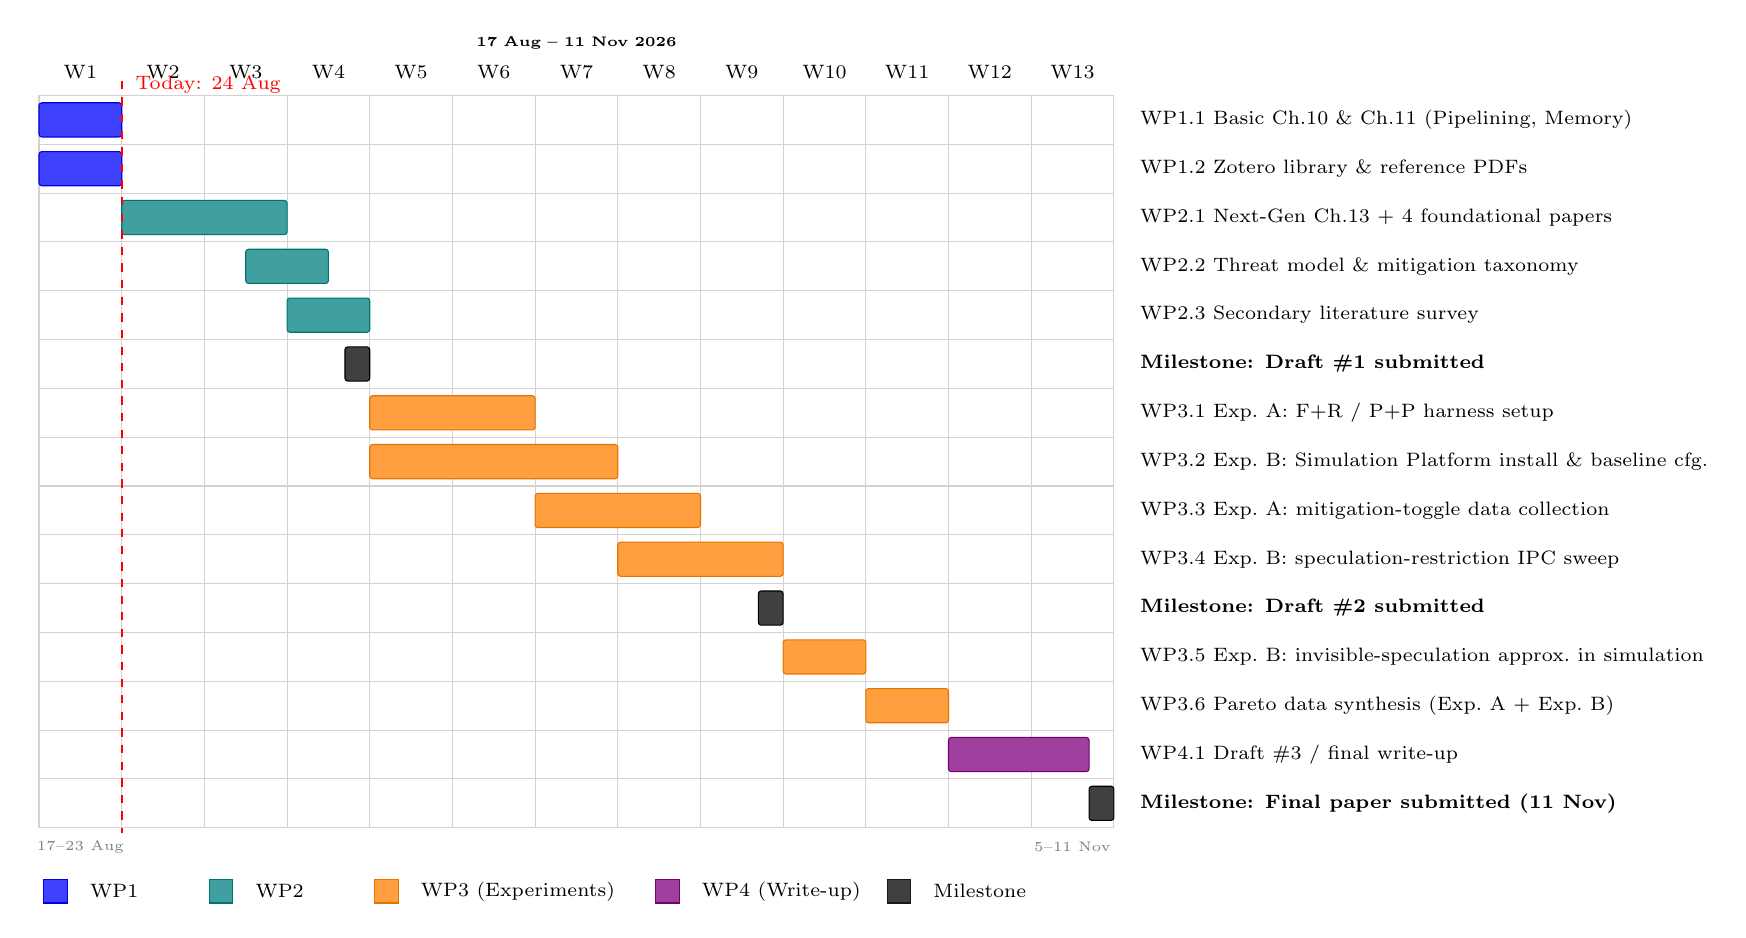
\begin{tikzpicture}[x=1.05cm,y=0.62cm]

% ---- parameters ----
% 13 week columns, 15 task rows

% Row labels (top to bottom), and (start,end,color,milestone?)
\def\nrows{15}

% Gridlines: vertical week separators
\foreach \w in {0,...,13} {
    \draw[gray!35] (\w,0) -- (\w,-\nrows);
}
\foreach \r in {0,...,\nrows} {
    \draw[gray!35] (0,-\r) -- (13,-\r);
}

% Week labels along top
\foreach \w [count=\i from 0] in
  {W1,W2,W3,W4,W5,W6,W7,W8,W9,W10,W11,W12,W13} {
    \node[font=\scriptsize,anchor=south] at (\i+0.5,0.15) {\w};
}
\node[font=\tiny,anchor=south,text width=13cm,align=center] at (6.5,0.75)
   {\textbf{17 Aug -- 11 Nov 2026}};

% Date sub-labels (approximate)
\node[font=\tiny,gray] at (0.5,-15.4) {17--23 Aug};
\node[font=\tiny,gray] at (12.5,-15.4) {5--11 Nov};

% ---- Task bars: \gbar{row}{start}{end}{colour}{label}
\newcommand{\gbar}[5]{
  \draw[fill=#4!75,draw=#4!90!black,rounded corners=1pt]
       (#2,-#1+0.15) rectangle (#3,-#1+0.85);
  \node[font=\scriptsize,anchor=west,text=black] at (13.2,-#1+0.5) {#5};
}
\newcommand{\ylabel}[2]{
  \node[font=\scriptsize,anchor=east] at (-0.15,-#1+0.5) {#2};
}

% WP1 - blue (Background / reference collection)
\gbar{1}{0}{1}{blue}{WP1.1 Basic Ch.10 \& Ch.11 (Pipelining, Memory)}
\gbar{2}{0}{1}{blue}{WP1.2 Zotero library \& reference PDFs}
% WP2 - teal (Literature / technical synthesis)
\gbar{3}{1}{3}{teal}{WP2.1 Next-Gen Ch.13 + 4 foundational papers}
\gbar{4}{2.5}{3.5}{teal}{WP2.2 Threat model \& mitigation taxonomy}
\gbar{5}{3}{4}{teal}{WP2.3 Secondary literature survey}
% Milestone - Draft 1
\gbar{6}{3.7}{4}{black}{\textbf{Milestone: Draft \#1 submitted}}
% WP3 - orange (Experiments: measurement, Tejas simulation, data collection)
\gbar{7}{4}{6}{orange}{WP3.1 Exp.\ A: F+R / P+P harness setup}
\gbar{8}{4}{7}{orange}{WP3.2 Exp.\ B: Simulation Platform install \& baseline cfg.}
\gbar{9}{6}{8}{orange}{WP3.3 Exp.\ A: mitigation-toggle data collection}
\gbar{10}{7}{9}{orange}{WP3.4 Exp.\ B: speculation-restriction IPC sweep}
% Milestone - Draft 2
\gbar{11}{8.7}{9}{black}{\textbf{Milestone: Draft \#2 submitted}}
% WP3 (cont.) - orange
\gbar{12}{9}{10}{orange}{WP3.5 Exp.\ B: invisible-speculation approx.\ in simulation}
\gbar{13}{10}{11}{orange}{WP3.6 Pareto data synthesis (Exp.\ A + Exp.\ B)}
% WP4 - violet (Write-up)
\gbar{14}{11}{12.7}{violet}{WP4.1 Draft \#3 / final write-up}
\gbar{15}{12.7}{13}{black}{\textbf{Milestone: Final paper submitted (11 Nov)}}

% Today marker
\draw[dashed,red,thick] (1,0.3) -- (1,-15.1);
\node[font=\scriptsize,red,anchor=south west] at (1.05,-0.15) {Today: 24 Aug};

% Legend
\node[draw=blue!90!black,fill=blue!75,minimum width=0.3cm,minimum height=0.3cm] at (0.2,-16.3) {};
\node[font=\scriptsize,anchor=west] at (0.5,-16.3) {WP1};
\node[draw=teal!90!black,fill=teal!75,minimum width=0.3cm,minimum height=0.3cm] at (2.2,-16.3) {};
\node[font=\scriptsize,anchor=west] at (2.5,-16.3) {WP2};
\node[draw=orange!90!black,fill=orange!75,minimum width=0.3cm,minimum height=0.3cm] at (4.2,-16.3) {};
\node[font=\scriptsize,anchor=west] at (4.5,-16.3) {WP3 (Experiments)};
\node[draw=violet!90!black,fill=violet!75,minimum width=0.3cm,minimum height=0.3cm] at (7.6,-16.3) {};
\node[font=\scriptsize,anchor=west] at (7.9,-16.3) {WP4 (Write-up)};
\node[draw=black!90,fill=black!75,minimum width=0.3cm,minimum height=0.3cm] at (10.4,-16.3) {};
\node[font=\scriptsize,anchor=west] at (10.7,-16.3) {Milestone};

\end{tikzpicture}}
\caption{Thirteen-week Gantt chart, 17 August -- 11 November 2026, broken into
granular sub-tasks across WP1--WP4. The dashed red line marks the current
reporting date, 24 August 2026. Bars for WP1 are complete; WP2 is in progress;
WP3 and WP4 are planned.}
\label{fig:gantt}
\end{figure}

\clearpage

\section{Technical Foundations Established}
\label{sec:techfound}

\subsection{Anatomy of an Out-of-Order Pipeline}
\label{sec:anatomy}

Before discussing why speculation is unavoidable and where it becomes a
security liability, it is worth fixing the pipeline vocabulary we use
throughout the rest of this report. Figure~\ref{fig:pipeline} sketches the
stages of a generic superscalar out-of-order core, as developed in Chapter~10
of the basic text~\cite{sarangi2025basic}: instructions are \emph{fetched}
from the instruction cache under the direction of the branch predictor,
\emph{decoded} and \emph{renamed} (architectural register names are mapped
onto physical registers, and an entry is allocated in the reorder buffer),
\emph{dispatched} into reservation stations where they wait for their
operands to become ready, \emph{issued} to a functional unit out of program
order as soon as operands and the unit are available, and finally
\emph{committed} from the head of the ROB strictly in program order once all
older instructions have committed and no exception or misprediction has been
detected for them. It is this last stage, commit, that is the sole point at
which microarchitectural work becomes architecturally visible; everything
before it is, by construction, speculative and reversible at the level of
registers and the ROB.

\begin{figure}[h]
\centering
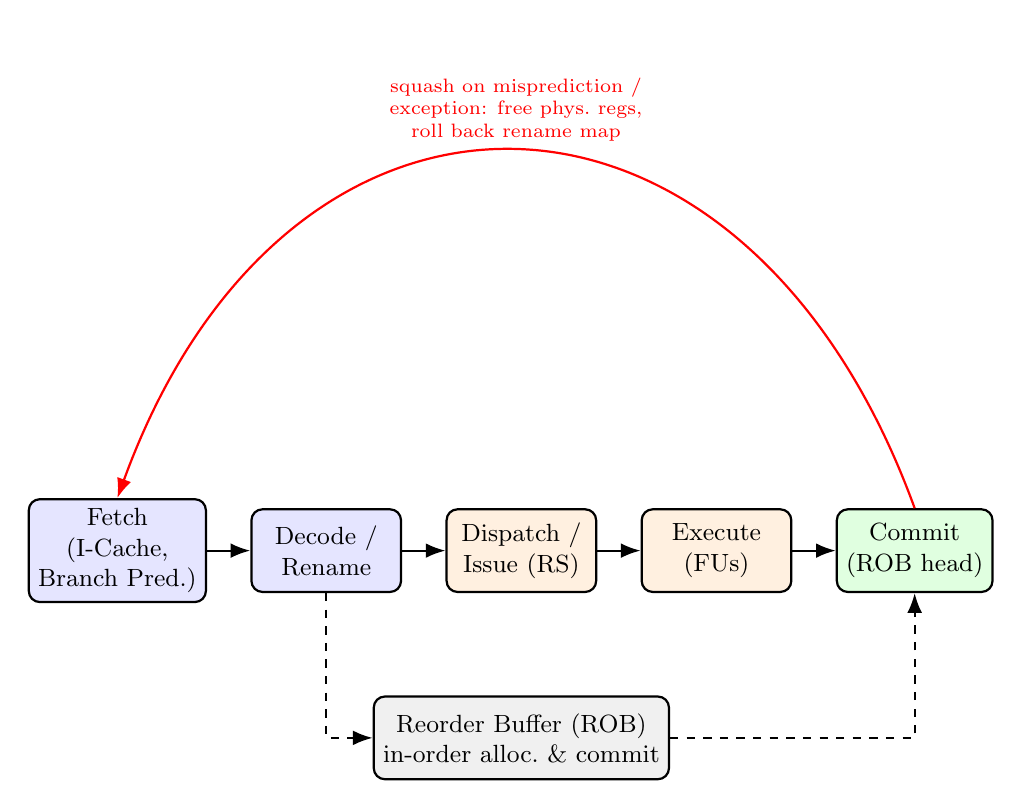
\begin{tikzpicture}[
  node distance=0.55cm and 0.55cm,
  stg/.style={draw,thick,rounded corners,minimum width=1.9cm,minimum height=1.05cm,align=center,font=\small},
  arr/.style={-{Latex[length=2.5mm]},thick}
]
\node[stg,fill=blue!10]  (fetch)   {Fetch\\(I-Cache,\\Branch Pred.)};
\node[stg,fill=blue!10,right=of fetch]  (decode)  {Decode /\\Rename};
\node[stg,fill=orange!12,right=of decode] (issue) {Dispatch /\\Issue (RS)};
\node[stg,fill=orange!12,right=of issue]  (exec)  {Execute\\(FUs)};
\node[stg,fill=green!12,right=of exec]  (commit) {Commit\\(ROB head)};

\draw[arr] (fetch) -- (decode);
\draw[arr] (decode) -- (issue);
\draw[arr] (issue) -- (exec);
\draw[arr] (exec) -- (commit);

\node[stg,fill=gray!12,below=1.3cm of issue,minimum width=3.4cm] (rob) {Reorder Buffer (ROB)\\ in-order alloc.\ \& commit};
\draw[arr,dashed] (decode.south) |- (rob.west);
\draw[arr,dashed] (rob.east) -| (commit.south);

\draw[arr,red,thick] (commit.north) to[out=110,in=70,looseness=1.6]
   node[above,font=\scriptsize,red,align=center]{squash on misprediction /\\exception: free phys.\ regs,\\roll back rename map} (fetch.north);
\end{tikzpicture}
\caption{Generic superscalar out-of-order pipeline. Instructions execute out
of program order between rename and commit, but the ROB enforces in-order
allocation and in-order commit, which is what makes the architectural rollback
on a squash (red path) precise. The rollback restores registers and the
rename map, but --- critically for our topic --- has no mechanism to undo
side effects already made in the cache hierarchy.}
\label{fig:pipeline}
\end{figure}

The key point that recurs throughout this report is the asymmetry visible in
Figure~\ref{fig:pipeline}: the squash path (red) is drawn only in terms of
pipeline-internal structures --- the ROB, the rename map, and the physical
register file --- because those are the only structures the ISA's rollback
contract was designed to cover. The functional units, in the course of
executing a load speculatively, will have already issued a request to the
cache hierarchy, and nothing in the squash mechanism reaches into the cache
to undo that request's side effects. The next two subsections develop
exactly why that omission is exploitable.

\subsection{Why Speculation Became Unavoidable}

The single most persistent trend in computer architecture over the last three
decades has been the widening gap between processor cycle time and main-memory
access latency. DRAM access latency, dominated by row-activation and bit-line
sensing physics rather than by transistor switching speed, has improved far more
slowly than logic performance. A last-level cache miss on a contemporary
server-class processor can cost on the order of 150--300 core clock cycles. If a
processor executed instructions strictly in program order and stalled the entire
pipeline on every such miss, an enormous fraction of available issue slots would
be wasted waiting on memory, and effective IPC would be governed almost entirely
by memory latency rather than by the machine's peak issue width.
Table~\ref{tab:latency} summarises the representative access latencies, drawn
from Chapter~11 of the basic text~\cite{sarangi2025basic}, that motivate this
design pressure and that will also directly calibrate the L1-hit/DRAM-miss
threshold we measure empirically in Experiment~A.

\begin{table}[h]
\centering
\begin{tabular}{@{}lcc@{}}
\toprule
\textbf{Structure} & \textbf{Typical Size} & \textbf{Typical Access Latency} \\
\midrule
L1 data cache & 32--48\,KB & 1--4 cycles \\
L2 cache & 256\,KB--1\,MB & 10--20 cycles \\
L3 / last-level cache (shared) & several MB & 30--70 cycles \\
Main memory (DRAM) & GBs & 150--300+ cycles \\
\bottomrule
\end{tabular}
\caption{Representative cache-hierarchy access latencies motivating
out-of-order, speculative execution as a latency-hiding mechanism. These
figures also fix the expected separability of the L1-hit/DRAM-miss
distributions we calibrate in Experiment~A (Section~\ref{sec:expA}).}
\label{tab:latency}
\end{table}

Out-of-order (OoO) execution is the architectural response to this problem.
Rather than blocking the whole pipeline on a stalled instruction, an OoO core
uses a reorder buffer (ROB), reservation stations, and register renaming to allow
independent instructions that appear later in program order to execute before an
earlier instruction that is stalled on a cache miss, provided the later
instructions do not have a true data dependence on the stalled one. This is
precisely the mechanism developed in the pipelining and out-of-order execution
material of the course text~\cite{sarangi2025basic}: the ROB preserves the
illusion of in-order commit for precise exceptions, and a scheduler (wake-up and
select logic) dynamically dispatches instructions to functional units as their
operands become ready.

Branch prediction is the second, and for our topic more consequential, half of
this story. Even with a large instruction window, a core cannot usefully look
ahead past an unresolved conditional branch unless it guesses which way the
branch will go and begins fetching and executing down the predicted path. Modern
branch predictors achieve prediction accuracies well above 95\% on typical
integer and floating-point workloads, which is precisely why the performance
gain from speculating past a branch outweighs, on average, the recovery cost of
a misprediction. Combined with hardware prefetchers that speculatively fetch
data before it is demanded, and memory-disambiguation logic that speculatively
allows loads to bypass earlier, address-unknown stores, a modern core is
speculative almost by default: at any instant a large fraction of the
instructions in flight in the ROB may never ultimately commit. This is the
load-bearing design decision our paper interrogates --- speculation is not a
peripheral optimisation that could be switched off cheaply; it is deeply
interwoven with how the pipeline hides memory latency and how the front end
sustains its fetch bandwidth, which is exactly why building a \emph{secure form
of speculation}, rather than simply disabling it, is the difficult and
interesting engineering problem.

Published characterisations of memory-latency-bound workloads consistently show
that disabling out-of-order issue and reverting to strict in-order execution can
cost a factor of two to four in IPC on memory-intensive benchmarks, while even
modest restrictions --- limiting how deep the core will speculate past an
unresolved branch, or serialising memory disambiguation --- have been reported
to cost anywhere from a few percent to over twenty percent IPC depending on
branch density and memory-level parallelism. This wide range is an important
finding for our paper: it suggests that the cost of security is a
workload-dependent curve rather than a single number, which is why we plan to
sweep multiple benchmarks and multiple speculation-restriction levels in
Experiment B (Section~\ref{sec:expB}).

\subsection{The Speculation Blind Spot}
\label{sec:blindspot}

The architectural contract of a modern OoO processor is that speculation is
invisible at the instruction set architecture (ISA) level: if a branch is
mispredicted, the instructions fetched down the wrong path are squashed from the
ROB and their register-renaming state is rolled back, so that architectural
registers and memory are left exactly as if those instructions had never
executed. Register renaming is central to this guarantee: by mapping
architectural register names onto a larger pool of \emph{physical} registers,
the renaming stage eliminates write-after-write (WAW) and write-after-read
(WAR) hazards that would otherwise force the pipeline to stall or serialise
independent instructions. On a squash, the physical registers allocated to the
mis-speculated instructions are simply freed and the rename map is rolled back
to the last correct checkpoint --- an operation that is cheap precisely because
it touches only renaming and ROB metadata, not the memory system.

This is also exactly where the guarantee breaks down. The rollback is
architecturally complete but \emph{microarchitecturally partial}: it restores
every piece of state that the ISA exposes (registers, memory, flags), but not
the state that the ISA was never designed to expose. Caches are the paradigmatic
example. When a speculatively executed load reads an address, the corresponding
line is installed into the L1 (and possibly L2/LLC) cache as a normal side
effect of servicing the memory request, exactly as described in the memory
system chapter of the course text~\cite{sarangi2025basic}. Squashing the
speculative load removes its effect on architectural registers, but it does
\emph{not} evict the cache line that load pulled in: cache eviction is governed
by the replacement policy (LRU, pseudo-LRU, or a variant) reacting to subsequent
accesses, not by pipeline squash logic. The result is that a \emph{transient
instruction} --- one that is fetched, executed, and eventually squashed, and
that therefore never architecturally happened --- can still leave a durable,
measurable footprint in the cache hierarchy.

This is precisely the mechanism exploited by Spectre-family
attacks~\cite{kocher2019spectre}. An attacker mistrains a branch predictor so
that the victim speculatively executes a bounds-check-bypassing load, using an
attacker-controlled out-of-bounds index to read secret data, and then uses that
secret byte to index a second, attacker-visible array. Even though the branch
misprediction is eventually detected and the entire speculative window is
squashed, the second array access has already changed which cache line of the
attacker's probe array is resident in the shared cache, and that change
survives the squash. Meltdown~\cite{lipp2018meltdown} exploits a closely
related but distinct blind spot: on affected processors, a load that should
raise a permission fault is nonetheless allowed to forward its result to
dependent, transiently executed instructions before the fault is
architecturally raised, again leaving a cache-resident footprint that encodes
the forbidden data. In both cases the structural cause is identical: the
hardware's notion of rollback is scoped to architectural state, while the
confidentiality properties programmers rely on implicitly assume that no
observable state should change as a result of computation the ISA says never
happened. Closing this blind spot without disabling speculation altogether is
the central design challenge surveyed in Chapter~13 of the primary
text~\cite{sarangi2023nextgen} and is the axis along which we evaluate
mitigation techniques in Section~\ref{sec:mitigations}.

The blind spot is not confined to the data cache. Any microarchitectural
structure whose state persists past a squash and whose occupancy is a function
of the (transient) instruction stream is, in principle, a candidate covert
channel: the branch-target buffer and pattern-history table (exploited directly
by Spectre Variant 2's predictor poisoning), the translation look-aside buffer,
and port contention in the execution back end have all been shown, in the
broader literature, to leak transient-execution side effects. We scope our own
experiments (Section~\ref{sec:expA}) to the cache-based channel, both because
it is the best-understood and most reproducible on commodity hardware available
to us, and because the memory-system background from Chapter~11 of the basic
text~\cite{sarangi2025basic} gives us the strongest foundation to reason about
it quantitatively.

\subsection{Cache-Timing Channels}
\label{sec:cachetiming}

To actually extract the secret-dependent cache footprint left behind by
transient execution, an attacker needs a way to convert \emph{is this cache
line resident or not} into a value measurable from unprivileged code. The
dominant technique used across the Spectre, Meltdown, and Foreshadow papers is
Flush+Reload, which exploits two properties of modern cache hierarchies: (i) an
unprivileged instruction such as \texttt{clflush} can evict a chosen line from
all levels of the cache, and (ii) the latency of a subsequent load to that same
address differs dramatically depending on whether the line has since been
reloaded --- an L1 hit takes on the order of a few cycles, whereas a DRAM-serviced
miss takes on the order of a few hundred cycles, a gap trivially resolvable with
the \texttt{rdtsc} timestamp-counter instruction. Figure~\ref{fig:flushreload}
illustrates the resulting attack loop.

\begin{figure}[h]
\centering
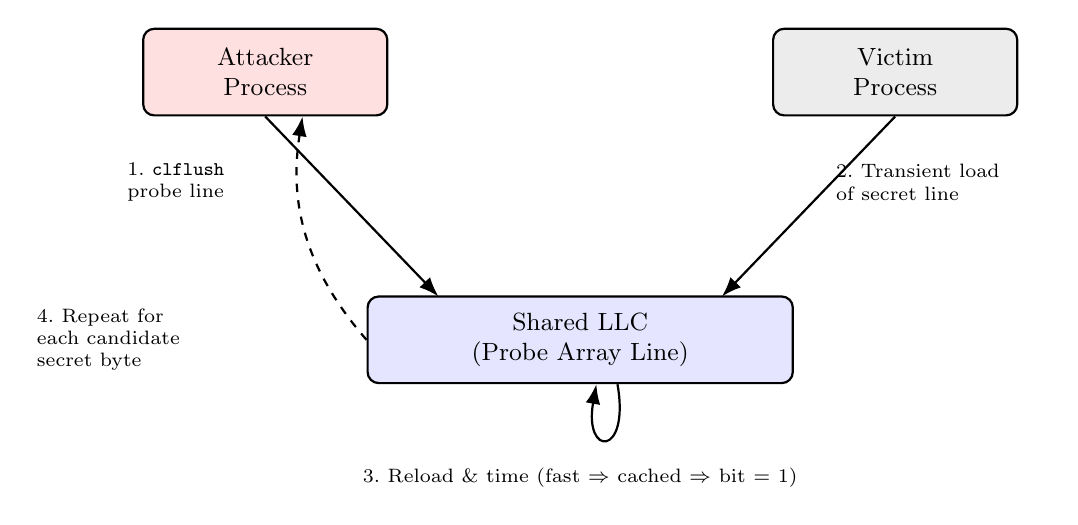
\begin{tikzpicture}[
  box/.style={draw,rounded corners,thick,minimum width=3.1cm,minimum height=1.1cm,align=center,font=\small},
  arr/.style={-{Latex[length=2.5mm]},thick},
  lbl/.style={font=\scriptsize,align=center}
]
\node[box,fill=red!12]  (attacker) at (0,5)    {Attacker\\Process};
\node[box,fill=gray!15] (victim)   at (8,5)    {Victim\\Process};
\node[box,fill=blue!10,minimum width=5.4cm] (cache) at (4,1.6) {Shared LLC\\(Probe Array Line)};

% Step 1: attacker flushes the line
\draw[arr] (attacker.south) -- (2.2,2.15);
\node[lbl,align=left,text width=2.4cm] at (-0.55,3.6) {1.\ \texttt{clflush}\\probe line};

% Step 2: victim transiently loads the secret-indexed line
\draw[arr] (victim.south) -- (5.8,2.15);
\node[lbl,align=left,text width=2.6cm] at (8.55,3.6) {2.\ Transient load\\of secret line};

% Step 3: attacker reloads and times (small self-loop below cache)
\draw[arr] (cache.310) to[out=280,in=260,looseness=9] (cache.290);
\node[lbl] at (4,-0.15) {3.\ Reload \& time (fast $\Rightarrow$ cached $\Rightarrow$ bit = 1)};

% Step 4: repeat for every candidate byte -- wide dashed loop on the far left
\draw[arr,dashed] (cache.west) to[bend left=25] (attacker.310);
\node[lbl,align=left,text width=2.4cm] at (-1.7,1.6) {4.\ Repeat for\\each candidate\\secret byte};

\end{tikzpicture}
\caption{The Flush+Reload attack loop between an attacker process, a shared
cache line, and a victim process. Steps~1--3 are repeated for every candidate
value of the secret, turning cache residency into a timing-measurable
one-byte covert channel.}
\label{fig:flushreload}
\end{figure}

The loop works as follows. In Step~1, the attacker evicts a chosen line of a
probe array (typically one line per possible byte value, 256 candidate lines)
using \texttt{clflush}. In Step~2, the victim is induced --- either through
normal program behaviour or, in the Spectre case, through a deliberately
mistrained branch --- to transiently access the probe-array line corresponding
to the secret byte's value, e.g.\ via an access pattern of the form
\texttt{probe\_array[secret\_byte * 4096]}, where the stride ensures each byte
value maps to a distinct, non-aliasing cache line. In Step~3, the attacker
times a reload of every candidate line; the line returning in L1-hit time
rather than DRAM-miss time reveals which line the victim touched, and hence the
secret byte's value. Step~4 repeats the procedure for every byte the attacker
wishes to exfiltrate. Published Spectre and Meltdown proof-of-concept
implementations demonstrate covert-channel bandwidths on the order of hundreds
of kilobytes per second on unmitigated hardware.

Flush+Reload requires a shared, coherent cache between attacker and victim and
the ability to execute \texttt{clflush}; Prime+Probe, an alternative channel we
compare it against in Experiment~A, relaxes both requirements by using
cache-set contention rather than line sharing, at the cost of a noisier signal.
Rowhammer~\cite{kim2014rowhammer}, by contrast, is not a cache-timing channel
at all --- it induces bit flips in neighbouring DRAM rows via repeated, uncached
row activations --- and we include it in our reading precisely as a contrast
case: it demonstrates that microarchitectural/physical-layer blind spots of
this general kind are not unique to caches or to speculation.

\subsection{Other Microarchitectural Covert Channels}
\label{sec:otherchannels}

Although our own experiments are scoped to the cache, the same rollback
asymmetry identified in Section~\ref{sec:blindspot} recurs across several
other structures, and we intend to discuss these qualitatively in the final
paper's related-work framing. Table~\ref{tab:channels} summarises the
channels we have identified in our reading so far, alongside the structure
each one exploits and the granularity of the signal it yields.

\begin{table}[h]
\centering
\begin{tabular}{@{}p{3.2cm}p{4.4cm}p{2.2cm}p{3.4cm}@{}}
\toprule
\textbf{Channel} & \textbf{Exploited Structure} & \textbf{Signal Granularity} & \textbf{Representative Use} \\
\midrule
Flush+Reload & Shared, inclusive LLC line & Byte-level & Spectre, Meltdown, Foreshadow \\
\addlinespace
Prime+Probe & Cache set contention & Byte-level (noisier) & Cross-VM cache attacks, no shared memory required \\
\addlinespace
Branch-target / pattern-history probing & BTB, PHT occupancy & Control-flow bit & Spectre Variant 2 predictor poisoning \\
\addlinespace
TLB-based channels & Translation look-aside buffer & Page-level & Address-translation side channels \\
\addlinespace
Port-contention channels & Execution-unit scheduler ports & Instruction-class bit & SMT co-tenant fingerprinting \\
\bottomrule
\end{tabular}
\caption{Comparative summary of microarchitectural covert channels discussed
in our secondary reading. Our own experimental work (Section~\ref{sec:exp})
is scoped to the first two rows.}
\label{tab:channels}
\end{table}

We restrict Experiment~A to Flush+Reload and Prime+Probe, both because they
are the best-understood and most reproducible on the commodity hardware
available to us, and because the memory-system background from Chapter~11 of
the basic text~\cite{sarangi2025basic} gives us the strongest quantitative
foundation to reason about them; the remaining rows of Table~\ref{tab:channels}
will be discussed qualitatively, from the secondary literature, in the final
paper.

\subsection{A Preliminary Taxonomy of Mitigations}
\label{sec:mitigations}

To orient the experimental plan in Section~\ref{sec:exp}, we conclude our
technical foundations with a preliminary taxonomy, drawn from Chapter~13 of the
primary text~\cite{sarangi2023nextgen}, of the broad strategies proposed to
close the speculation blind spot. We group them by where in the pipeline they
intervene, since this correlates strongly with the performance cost each
strategy is expected to impose. Table~\ref{tab:taxonomy} summarises the four
strategies identified so far.

\begin{table}[h]
\centering
\begin{tabular}{@{}p{2.6cm}p{5.2cm}p{2cm}p{3.4cm}@{}}
\toprule
\textbf{Strategy} & \textbf{Mechanism} & \textbf{Intervention Point} & \textbf{Expected Cost Profile} \\
\midrule
Fencing / serialisation & Explicit instructions (e.g.\ \texttt{LFENCE}) or compiler-inserted barriers that block speculation past a sensitive branch entirely & Software / ISA & High, localised (each fence stalls the front end) \\
\addlinespace
Invisible speculation & Delay the visible microarchitectural effect of a speculative memory access until the access is known to be non-speculative & Cache / memory hierarchy & Moderate, broad (adds latency to every load) \\
\addlinespace
Partitioning / randomisation & Statically or dynamically partition cache ways, or randomise the address-to-set mapping, so attacker and victim cannot alias the same structures & Cache hierarchy & Moderate, capacity-dependent \\
\addlinespace
Taint tracking & Tag speculatively loaded, not-yet-committed data as tainted and block tainted values from influencing observable structures until resolved & Pipeline / renaming logic & Low--moderate, but adds datapath and verification complexity \\
\bottomrule
\end{tabular}
\caption{Preliminary taxonomy of mitigation strategies for cache-timing side
channels arising from speculative execution.}
\label{tab:taxonomy}
\end{table}

Production mitigations against Spectre and Meltdown span more than one row of
this taxonomy. Retpolines are a targeted, software-level instance of the
fencing/serialisation row, inserting return-trampoline sequences that block
branch-target injection without new hardware. Kernel page-table isolation
(KPTI), by contrast, is \emph{not} a fencing or serialisation mechanism: it is
an operating-system defence that removes the kernel's address-space mapping from
user-mode page tables, closing the specific Meltdown fault-order path into kernel
memory rather than restricting speculation anywhere in the pipeline. Both were
adopted because they could be deployed on existing silicon, whereas the
invisible-speculation and taint-tracking schemes remain largely confined to the
research literature because they require microarchitectural changes not yet
adopted at scale.

\subsection{Framing the Cost in Power-Performance-Area Terms}
\label{sec:ppa}

Experiment~B, as scoped in Section~\ref{sec:expB}, measures the cost of
mitigation purely in IPC. IPC is the right primary metric for a course-length
simulation study because it is directly observable from simulation platform without
modelling silicon implementation details, but it is only one axis of the
power-performance-area (PPA) budget that actually governs whether a vendor
ships a given defence. Table~\ref{tab:taxonomy}'s ``expected cost profile''
column already hints at this: fencing costs cycles but essentially no extra
area, since it reuses existing pipeline flush logic; invisible speculation
costs both cycles (extra latency on every load) and area (buffering to hold
the not-yet-visible cache state); partitioning costs effective cache
capacity, which is itself a PPA trade against building a larger physical
cache; and taint tracking costs verification complexity and datapath area
(extra tag bits that must be threaded through the renaming and forwarding
logic) more than raw cycles. We do not have the tooling in this course
project to measure area or power directly --- that would require a physical
design flow beyond our scope --- but we intend to use the qualitative PPA
framing above, together with the mitigation taxonomy of
Table~\ref{tab:taxonomy}, to interpret our IPC results in Q4's terms: a
defence that costs little IPC but a great deal of verification and area
complexity can still be commercially unattractive even though our
simulation-only view of the trade-off would report it favourably. We plan to
flag this limitation explicitly wherever we discuss Experiment~B's results in
Draft~\#2 and the final paper.

\clearpage

\section{Literature Review}
\label{sec:litreview}

Our reading has grown beyond the four foundational papers named in Task~WP2.1
to cover the wider transient-execution literature. To keep the reference set
focused rather than uniformly weighted, we distinguish \emph{core} references
--- the ten papers our threat model, mitigation taxonomy, and experimental
design depend on directly --- from \emph{supporting} references that we cite for
completeness but do not build on. Table~\ref{tab:coremap} maps each core
reference to the work package it belongs to, the specific mechanism or datum we
extract from it, and where in the project it is used; the supporting references
are listed compactly beneath it. We reserve longer prose below for the core
attack and defence papers only.

\subsection{Foundational Attack Papers}
\label{sec:foundational}

\textbf{Spectre~\cite{kocher2019spectre}} gives the attack template that
names the whole family: an attacker mistrains a predictor (branch-target
buffer, pattern-history table, or return-address stack) so that a victim's
speculative execution path touches data the attacker should not have access
to, and the resulting change in cache residency is recovered via a timing
side channel. Its two variants --- bounds-check bypass and branch-target
injection --- are the direct ancestors of nearly every attack we discuss
below, and its central claim, that no single instruction is at fault, is why
Spectre-class mitigations have proven so hard to retrofit.

\textbf{Meltdown~\cite{lipp2018meltdown}} shows that on several Intel (and
some other) processors, a load's result is forwarded to dependent transient
instructions before a permission fault on that load is architecturally
raised, letting unprivileged code read kernel memory and exfiltrate it via
Flush+Reload. Because the defect is an ordering bug rather than a mistrained
predictor, it was fixable at the OS level by page-table isolation (KPTI) at a measured cost --- our
paper's first concrete instance of the performance-for-security trade-off.

\textbf{Foreshadow~\cite{vanbulck2018foreshadow}} extends the Meltdown-style
L1-terminal-fault mechanism to Intel SGX enclaves, showing that hardware
memory encryption does not stop a transient read if the underlying L1 cache
is shared with an untrusted context. This broadens the practical stakes of
Experiment~B, since enclave workloads are the class of application least able
to tolerate a compromised boundary.

\textbf{Rowhammer~\cite{kim2014rowhammer}} predates the other three by
several years and is not a speculative or cache-timing attack at all: it
shows that hammering a DRAM row can flip bits in adjacent rows through charge
leakage alone. We keep it as a contrast case rather than a direct object of
study, establishing that ISA-invisible microarchitectural blind spots are a
broader pattern in computer architecture, not a speculation-specific one.

\subsection{Systematisation and Measurement}

\textbf{Canella et al.~\cite{canella2019systematic}} systematise the
Spectre and Meltdown families into a single classification tree, using it to
uncover several previously overlooked attack variants and to show that most
deployed defences, including KPTI and retpolines, leave part of the attack
surface open. We use this classification, rather than an attack-by-attack
narrative, to frame the ``family'' language throughout Section~\ref{sec:techfound}.

\textbf{Yarom and Falkner~\cite{yarom2014flushreload}} introduced Flush+Reload
itself, four years before Spectre, as a page-deduplication attack on the
last-level cache; nearly every proof-of-concept transient-execution attack
since has reused it unmodified as the readout primitive, which is why we treat
it as foundational rather than secondary.

\subsection{Hardware Defence Proposals}

Three core papers instantiate rows of our mitigation taxonomy
(Table~\ref{tab:taxonomy}) as concrete microarchitecture.
\textbf{InvisiSpec}~\cite{yan2018invisispec} delays a speculative load's effect
on the cache hierarchy until the load is known non-speculative, reporting a
slowdown of 21\% against an unmitigated baseline (versus 74\% for naive fencing)
under a Spectre threat model, and is the defence we plan to approximate in
Experiment~B. \textbf{Speculative Taint Tracking (STT)}~\cite{yu2019stt} instead
tags speculatively loaded values and blocks only the propagation of tainted data
to observable channels, aiming for the taint-tracking row's lower cost profile.
\textbf{DAWG}~\cite{kiriansky2018dawg} statically partitions cache ways into
protection domains so that an attacker and victim in different domains cannot
alias the same set, instantiating the partitioning row.

\begin{table}[h]
\centering
\small
\begin{tabular}{@{}p{3.3cm}p{1.2cm}p{4.3cm}p{4.1cm}@{}}
\toprule
\textbf{Core Reference} & \textbf{WP} & \textbf{Mechanism / data extracted} & \textbf{Where used in our project} \\
\midrule
Spectre~\cite{kocher2019spectre} & WP2 & Branch-predictor mistraining drives a transient bounds-check bypass; supplies the cache-residency readout template & Blind-spot analysis (\S\ref{sec:blindspot}); threat model for Exp.\ A \\
\addlinespace
Meltdown~\cite{lipp2018meltdown} & WP2 & Fault-order defect forwards a faulting load's result to transient instructions before the fault is raised & Blind-spot analysis (\S\ref{sec:blindspot}); motivates the KPTI cost discussion \\
\addlinespace
Rowhammer~\cite{kim2014rowhammer} & WP2 & Physical DRAM row-hammering flips bits in adjacent rows (not transient-execution, not cache-timing) & Physical-disturbance \emph{contrast case} (\S\ref{sec:cachetiming}, \S\ref{sec:foundational}) \\
\addlinespace
Foreshadow~\cite{vanbulck2018foreshadow} & WP2 & L1 terminal fault enables a transient read of SGX enclave data & Extends threat model to the enclave boundary (\S\ref{sec:foundational}) \\
\addlinespace
Flush+Reload~\cite{yarom2014flushreload} & WP2 $\to$ WP3 & \texttt{clflush} plus a timed reload turns cache residency into a byte-level covert channel & Readout primitive built and calibrated in Exp.\ A (\S\ref{sec:expA}) \\
\addlinespace
Canella et al.~\cite{canella2019systematic} & WP2 & Classification tree of transient-execution attacks/defences; coverage gaps of deployed patches & Frames the ``family'' taxonomy language (\S\ref{sec:techfound}) \\
\addlinespace
InvisiSpec~\cite{yan2018invisispec} & WP2 $\to$ WP3 & Delays a speculative load's cache-visible effect until it is non-speculative (reported 21\% slowdown) & Invisible-speculation taxonomy row; approximated in Exp.\ B (\S\ref{sec:expB}) \\
\addlinespace
STT~\cite{yu2019stt} & WP2 & Tags speculatively-loaded data and blocks tainted propagation to observable channels & Taint-tracking row of the taxonomy (\S\ref{sec:mitigations}) \\
\addlinespace
DAWG~\cite{kiriansky2018dawg} & WP2 & Statically partitions cache ways into protection domains to prevent attacker--victim aliasing & Partitioning row of the taxonomy (\S\ref{sec:mitigations}) \\
\addlinespace
Retpoline~\cite{turner2018retpoline} & WP2 $\to$ WP3 & Return-trampoline software construct that blocks branch-target injection (Spectre-V2) & Software fencing instance; patched-vs-unpatched toggle in Exp.\ A \\
\bottomrule
\end{tabular}
\caption{Core references mapped to their owning work package, the mechanism or
datum extracted from each, and where each is used in the project. ``WP2 $\to$
WP3'' marks papers read and synthesised in WP2 that also directly feed an
experiment in WP3.}
\label{tab:coremap}
\end{table}

\subsection{Positioning and the Chronological Arc}

Read together, the literature above traces a coherent arc. Rowhammer (2014)
and Flush+Reload (2014) independently established, years before Spectre and
Meltdown, that ISA-invisible hardware effects --- one physical, one
microarchitectural --- could be turned into reliable attack primitives, but
neither was yet connected to speculative execution. Spectre and Meltdown
(2018) then showed that the far more pervasive mechanism of speculative,
out-of-order execution has an analogous invisible-at-the-ISA side effect,
exploitable via Flush+Reload on essentially every high-performance processor.
Foreshadow (2018) extended the same mechanism to hardware features explicitly
designed to resist a malicious privileged software stack, while
Canella et al.'s systematisation (2019) drew the resulting sprawl of variants
into a single classification tree. Against this, the defence literature
instantiates our mitigation taxonomy directly: InvisiSpec, DAWG, and STT all
appear within eighteen months of Spectre's disclosure, evidence of how
quickly architecture research mobilised once the attack surface was public.

Table~\ref{tab:variants} records the specific attack variants and follow-on
disclosures encountered while surveying secondary references, classified by
the mechanism each one exploits; the first four rows correspond to our
foundational readings above, and the MDS row is now backed by the primary
sources reviewed in Section~3.2 rather than only secondary mentions.

\begin{table}[h]
\centering
\begin{tabular}{@{}p{2.6cm}p{4.6cm}p{5.6cm}@{}}
\toprule
\textbf{Family} & \textbf{Mechanism Exploited} & \textbf{Notes} \\
\midrule
Spectre-V1 & Conditional branch mistraining (bounds-check bypass) & Requires an exploitable gadget in victim code; mitigated with fencing or bounds masking \\
\addlinespace
Spectre-V2 & Indirect branch / BTB poisoning & Cross-domain; mitigated with retpolines or indirect branch restricted speculation \\
\addlinespace
Meltdown (V3) & Fault-order defect on faulting loads & Fixed by KPTI at a measured TLB-flush cost \\
\addlinespace
Foreshadow (L1TF) & L1 terminal fault inside SGX & Extends the blind spot to enclave-protected memory \\
\bottomrule
\end{tabular}
\caption{Classification of transient-execution attack variants encountered
in our reading, by exploited mechanism.}
\label{tab:variants}
\end{table}

We see the value of our own contribution less in proposing a new attack or
defence --- outside the scope of a course project --- and more in producing a
grounded, quantitative comparison of the security-performance trade-off using
both real-hardware measurement and architectural simulation side by side,
something the literature above tends to address from only one of these two
angles at a time.

\clearpage

\section{Research Questions and Experimental Plan}
\label{sec:exp}

Building on the technical foundations above, we plan to answer our central
research question --- whether speculative execution can be secured against
cache-timing side channels without forfeiting its performance benefit ---
through two complementary experiments: one empirical, run on real x86
hardware, and one based on cycle-level architectural simulation. Real-hardware
measurement (Experiment~A) gives us ground-truth evidence that the attack side
channel is genuinely exploitable on hardware we can access, but commodity
processors do not expose most of the fine-grained speculation-control knobs
that a defence proposal like invisible speculation would require. Architectural
simulation (Experiment~B) gives us exactly that configurability, at the cost of
a timing model that is only as trustworthy as the simulator itself. Running
both, and being explicit about where their conclusions agree and diverge, is
our attempt to give a more defensible answer to the central research question
than either method could support on its own.

\subsection{Experiment A: Empirical Cache-Timing Litmus Tests on x86 Hardware}
\label{sec:expA}

The goal of Experiment~A is to establish, on real hardware available to us, a
calibrated, ground-truth measurement of the L1-hit versus DRAM-miss timing gap
that underlies Flush+Reload, and to use that calibration to build a minimal,
ethically-scoped covert channel between two cooperating processes on the same
machine. Concretely we plan to:

\begin{enumerate}[nosep]
\item Use \texttt{rdtsc}/\texttt{rdtscp} to build a histogram of access
latencies for L1 hits, LLC hits, and DRAM misses, establishing a threshold
that separates \emph{cached} from \emph{not cached} with high confidence.
\item Implement a minimal Flush+Reload covert channel between a sender and
receiver process sharing a memory-mapped file, and measure achievable
bit-error rate and bandwidth as a function of probe-array stride and
measurement threshold.
\item Repeat the measurement with mitigations relevant to a \emph{user-to-user}
Flush+Reload channel enabled versus disabled where our test environment allows
(e.g.\ restricted/serialised \texttt{rdtsc} access, cache way-partitioning via
Intel CAT, disabling the shared memory-mapped page or memory deduplication that
supplies the shared line, and hardware-prefetcher settings), to obtain an
empirical estimate of how much each degrades channel bandwidth. We deliberately
exclude kernel page-table isolation (KPTI) here: it isolates kernel memory from
user code and therefore does not affect a covert channel that operates entirely
between two unprivileged user processes sharing a memory-mapped region.
\end{enumerate}

This experiment directly exercises the memory-system material from
Chapter~11 of the basic text~\cite{sarangi2025basic} and grounds the
qualitative attack description of Section~\ref{sec:techfound} in quantitative,
hardware-measured numbers.

\subsection{Experiment B: Quantitative Simulation Using the Cycle - Level Architecture Simulator}
\label{sec:expB}

Where Experiment~A measures the attack side of the trade-off, Experiment~B is
designed to measure the defence side: the performance cost of closing the
speculation blind spot. Using a cycle-level architectural simulation platform, we plan to:

\begin{enumerate}[nosep]
\item Configure a baseline out-of-order core model in the simulation platform matching, as
closely as the platform allows, a contemporary superscalar pipeline
(multi-issue, ROB-based, with a realistic branch predictor and a two- or
three-level cache hierarchy), and run a representative subset of memory-latency-sensitive
benchmarks to obtain baseline IPC.
\item Re-run the same benchmarks with speculation restricted or disabled in
stages: first disabling speculative memory disambiguation, then restricting
branch-predictor-driven speculative depth, and finally emulating a fully
non-speculative execution mode, to build an IPC-versus-speculation-depth
curve.
\item Where configuration options permit, approximate an invisible-speculation-style
defence (e.g.\ delaying the visible effect of a speculative load on the cache
until the corresponding branch resolves) and measure the resulting IPC delta
relative to both the unmitigated baseline and the fully non-speculative
extreme.
\item Vary the benchmark mix to include both memory-latency-bound and
compute-bound workloads, since our reading (Section~\ref{sec:techfound})
suggests the IPC cost of restricting speculation should scale with a
workload's cache-miss rate and branch density.
\end{enumerate}

The intended output of Experiment~B is a quantitative IPC-degradation curve
that lets us state, in the final paper, not just \emph{that} security costs
performance but \emph{how much}. Combined with Experiment~A's empirical
channel-bandwidth measurements, this will let us frame our final conclusion
as an explicit security-performance Pareto curve rather than a qualitative
judgement. Table~\ref{tab:benchmarks} lists the provisional benchmark mix we
intend to use, chosen to separate memory-latency-bound behaviour from
compute-bound behaviour as motivated in Section~\ref{sec:techfound}.

\begin{table}[h]
\centering
\begin{tabular}{@{}p{3.4cm}p{4.4cm}p{5.4cm}@{}}
\toprule
\textbf{Class} & \textbf{Provisional Benchmarks} & \textbf{Rationale} \\
\midrule
Memory-latency-bound & \texttt{mcf}, \texttt{lbm}, \texttt{libquantum}-style kernels & High LLC miss rate; expected to show the largest IPC sensitivity to speculation restriction \\
\addlinespace
Compute-bound & \texttt{bzip2}, matrix-multiply / DSP-style kernels & Low miss rate; expected to isolate the fixed, branch-density-driven cost of fencing/serialisation \\
\addlinespace
Branch-heavy & Parser / interpreter-style kernels & Stresses the branch predictor and BTB-related mitigations specifically \\
\bottomrule
\end{tabular}
\caption{Provisional benchmark mix for Experiment~B, to be finalised once
the simulation build and its supported benchmark harness are confirmed.}
\label{tab:benchmarks}
\end{table}

\subsection{Metrics We Plan to Report}

To keep Experiments~A and~B directly comparable, and to avoid the common
pitfall of reporting attack and defence results in incommensurable units, we
plan to standardise on the following metrics. For Experiment~A: (i)
\emph{effective channel throughput}, in effective bits per second of the Flush+Reload
covert channel under a fixed, stated bit-error-rate tolerance; (ii)
\emph{measurement separability}, expressed as the statistical distance
between the cache-hit and cache-miss latency distributions, as a proxy for
how reliably an attacker could exploit the channel in practice; and (iii),
where a mitigation toggle is available, the \emph{relative channel
degradation}, i.e.\ the percentage reduction in (i) with the mitigation
enabled versus disabled. For Experiment~B: (i) baseline and mitigated IPC,
per benchmark; (ii) \emph{relative IPC degradation}, i.e.\ the percentage IPC
loss attributable to each speculation-restriction level relative to the
unmitigated baseline; and (iii), where feasible, an approximate
security-normalised performance figure that combines (ii) with the
corresponding channel degradation from Experiment~A for a comparable
mitigation, letting us plot a single security-performance Pareto curve rather
than two disconnected sets of numbers.

\subsection{Reproducibility Plan}

For Experiment~A, we plan to script the entire measurement pipeline ---
latency calibration, covert-channel encoding and decoding, and mitigation
toggling --- so that a run can be repeated with a single command, with raw
timing samples (not just summary statistics) logged to a file; this lets us
re-derive different metrics after the fact and report run-to-run variance
across repeated trials, which we consider necessary given how sensitive
cache-timing measurements are to background system load. For Experiment~B, we plan to keep every simulation configuration file used for a reported IPC
number under version control, together with the exact benchmark inputs and
simulator build identifier... This
matters in particular for the invisible-speculation-style approximation
described in Section~\ref{sec:mitigations}, since that configuration will
necessarily involve judgment calls about how to map a hardware defense
proposal onto the simulator's available knobs, and we want that mapping to be
audit-able rather than described only in prose.

\subsection{Success Criteria and Principal Risks}

We define success at three increasing levels of ambition, so that a partial
result at Draft~\#2 or Draft~\#3 still constitutes meaningful progress.
Table~\ref{tab:success} restates these levels alongside the concrete
deliverable and expected report.

\begin{table}[h]
\centering
\begin{tabular}{@{}p{2cm}p{7.8cm}p{3cm}@{}}
\toprule
\textbf{Level} & \textbf{Concrete Deliverable} & \textbf{Expected By} \\
\midrule
Minimum viable & Calibrated Flush+Reload measurement on real hardware; baseline, uncontested simulation IPC for at least two benchmarks & Draft \#2 \\
\addlinespace
Target & Above, plus one measured mitigation configuration in each experiment (an OS-level toggle for Exp.\ A; a speculation-restriction level for Exp.\ B) & Draft \#2 / early Draft \#3 \\
\addlinespace
Stretch & Above, plus a simulation approximation of an invisible-speculation-style defence with an attributable IPC cost, enabling a direct quantitative answer to the central research question & Draft \#3 / final paper \\
\bottomrule
\end{tabular}
\caption{Success criteria for the experimental plan, by level of ambition.}
\label{tab:success}
\end{table}

We have identified three principal risks. First, \emph{hardware access and
mitigation visibility}: not every OS/hardware combination we have access to
exposes the fine-grained mitigation toggles needed for Experiment~A; where a
toggle is unavailable we will fall back to comparing patched versus unpatched
kernel versions, or report the limitation explicitly. Second, \emph{simulator
fidelity}: our chosen architectural simulation platform models a specific,
simplified core configuration and may not expose all the speculation-control
knobs our plan requires; we have budgeted time to read the platform's
configuration documentation and implement configuration-level modifications
rather than modifying source code, to keep the change within scope for a
term paper. Third, \emph{measurement noise}: cache-timing measurements on real
hardware are sensitive to system noise; we plan to control for this by
disabling frequency scaling and hyperthreading where possible and by
reporting distributions rather than single-sample timings, consistent with
standard practice in the side-channel literature. Fourth, \emph{simulator
scope creep}: because the simulation platform exposes a large number of configuration
parameters, there is a real risk of spending disproportionate time tuning the
baseline model rather than collecting the speculation-restriction sweep that
actually answers Q3; we mitigate this by using a pre-validated
out-of-order baseline configuration provided with the simulator
as our starting point rather than building a core model from scratch, and by fixing
a hard time-box for baseline tuning before moving on to the mitigation
sweeps.

\section{Summary of Progress and Next Steps}

As of 24 August 2026, WP1 is fully complete: we have read the assigned
Pipelining and Memory System chapters of the basic text~\cite{sarangi2025basic},
and have built a Zotero reference library containing our four foundational
papers plus both course textbooks. WP2 is in progress: we have substantially
completed a close reading of Spectre~\cite{kocher2019spectre},
Meltdown~\cite{lipp2018meltdown}, Rowhammer~\cite{kim2014rowhammer}, and
Foreshadow~\cite{vanbulck2018foreshadow}, and have used them, together with
Chapter~13 of the primary text~\cite{sarangi2023nextgen}, to write the
technical foundations and literature review in Sections~\ref{sec:techfound}
and~\ref{sec:litreview} of this report.

Our immediate next steps, to be reported in Draft~\#2, are to: finalise the
hardware/software configuration for Experiment~A; obtain a working cycle - level simulation
build and baseline IPC numbers for Experiment~B; and continue surveying the
secondary mitigation literature (speculative taint tracking, invisible
speculation, and cache-partitioning schemes) in more depth for the paper's
discussion section.

\section{Provisional Structure of the Final Term Paper}
\label{sec:outline}

Although this draft is scoped strictly to work completed as of 24 August
2026, it is useful --- both for our own planning and for the advisor's
review --- to record the provisional chapter structure we intend the
$\sim$150-page final term paper to grow into. Table~\ref{tab:outline} maps
each planned chapter onto the WP referenced in Table~\ref{tab:tasks} and the
Gantt chart of Figure~\ref{fig:gantt}, and is explicitly a forward-looking
plan rather than a commitment: chapter boundaries and page budgets will be
revised in Draft~\#2 once Experiment~A and Experiment~B results are
available to inform how much space each topic actually warrants.

\begin{table}[h]
\centering
\begin{tabular}{@{}p{1.2cm}p{5.4cm}p{5.4cm}p{1.6cm}@{}}
\toprule
\textbf{Ch.} & \textbf{Working Title} & \textbf{Content} & \textbf{Fed by} \\
\midrule
1 & Introduction to Microarchitectural Security & Problem statement; logical vs.\ physical isolation; timeline from cryptographic timing attacks to transient execution & WP1 \\
\addlinespace
2 & The Engines of Vulnerability & Out-of-order execution, branch prediction, and the cache hierarchy as the mechanisms that make speculation both fast and leaky (this draft's Section~\ref{sec:techfound}) & WP1, WP2 \\
\addlinespace
3 & The Threat Landscape & Anatomy of a side channel; Flush+Reload / Prime+Probe / Evict+Time; case studies of Spectre and Meltdown (this draft's Sections~\ref{sec:cachetiming}, \ref{sec:litreview}) & WP2 \\
\addlinespace
4 & Advanced Vulnerabilities in Main Memory & DRAM microarchitecture; the Rowhammer disturbance effect; Foreshadow and enclave-level threats & WP2 \\
\addlinespace
5 & Hardware Mitigations \& Secure Architectures & Fencing, invisible speculation, partitioning, taint tracking; why software-only patches (KPTI, retpolines) cost performance (this draft's Section~\ref{sec:mitigations}) & WP2, WP3 \\
\addlinespace
6 & Methodology, Simulation, and PPA Trade-offs & Experiment~A and Experiment~B design, execution, and results; the security-performance Pareto curve (this draft's Section~\ref{sec:exp}) & WP3 \\
\addlinespace
7 & Conclusion and Future Outlook & Answering Q1--Q4; open hardware (RISC-V) as a path to ground-up secure design & WP4 \\
\bottomrule
\end{tabular}
\caption{Provisional chapter structure for the final term paper, mapped to
the work packages and experiments already introduced in this draft.}
\label{tab:outline}
\end{table}

The technical foundations and literature review already written for this
draft (Sections~\ref{sec:techfound} and~\ref{sec:litreview}) are intended to
seed Chapters~2--4 directly, so that the writing effort in WP4 is
concentrated on new material --- principally the mitigation deep-dive of
Chapter~5 and the results chapter, Chapter~6, which cannot be written until
Experiments~A and~B have produced data.

\clearpage

\begin{thebibliography}{9}

\bibitem{sarangi2025basic}
S.~R. Sarangi, \textit{Basic Computer Architecture}. McGraw Hill Education, 2025.

\bibitem{sarangi2023nextgen}
S.~R. Sarangi, \textit{Next-Gen Computer Architecture}. McGraw Hill Education, 2023.

\bibitem{kocher2019spectre}
P.~Kocher, J.~Horn, A.~Fogh, D.~Genkin, D.~Gruss, W.~Haas, M.~Hamburg, M.~Lipp,
S.~Mangard, T.~Prescher, M.~Schwarz, and Y.~Yarom, ``Spectre Attacks: Exploiting
Speculative Execution,'' in \textit{Proceedings of the 40th IEEE Symposium on
Security and Privacy (S\&P)}, San Francisco, CA, USA, 2019, pp.~1--19.

\bibitem{lipp2018meltdown}
M.~Lipp, M.~Schwarz, D.~Gruss, T.~Prescher, W.~Haas, A.~Fogh, J.~Horn,
S.~Mangard, P.~Kocher, D.~Genkin, Y.~Yarom, and M.~Hamburg, ``Meltdown: Reading
Kernel Memory from User Space,'' in \textit{Proceedings of the 27th USENIX
Security Symposium}, Baltimore, MD, USA, 2018, pp.~973--990.

\bibitem{kim2014rowhammer}
Y.~Kim, R.~Daly, J.~Kim, C.~Fallin, J.~H. Lee, D.~Lee, C.~Wilkerson, K.~Lai,
and O.~Mutlu, ``Flipping Bits in Memory Without Accessing Them: An
Experimental Study of DRAM Disturbance Errors,'' in \textit{Proceedings of the
41st Annual International Symposium on Computer Architecture (ISCA)},
Minneapolis, MN, USA, 2014, pp.~361--372.

\bibitem{vanbulck2018foreshadow}
J.~Van Bulck, M.~Minkin, O.~Weisse, D.~Genkin, B.~Kasikci, F.~Piessens,
M.~Silberstein, T.~F. Wenisch, Y.~Yarom, and R.~Strackx, ``Foreshadow:
Extracting the Keys to the Intel SGX Kingdom with Transient Out-of-Order
Execution,'' in \textit{Proceedings of the 27th USENIX Security Symposium},
Baltimore, MD, USA, 2018, pp.~991--1008.

\bibitem{yarom2014flushreload}
Y.~Yarom and K.~Falkner, ``FLUSH+RELOAD: A High Resolution, Low Noise, L3
Cache Side-Channel Attack,'' in \textit{Proceedings of the 23rd USENIX
Security Symposium}, San Diego, CA, USA, 2014, pp.~719--732.

\bibitem{canella2019systematic}
C.~Canella, J.~Van Bulck, M.~Schwarz, M.~Lipp, B.~von Berg, P.~Ortner,
F.~Piessens, D.~Evtyushkin, and D.~Gruss, ``A Systematic Evaluation of
Transient Execution Attacks and Defenses,'' in \textit{Proceedings of the
28th USENIX Security Symposium}, Santa Clara, CA, USA, 2019, pp.~249--266.

\bibitem{yan2018invisispec}
M.~Yan, J.~Choi, D.~Skarlatos, A.~Morrison, C.~W. Fletcher, and J.~Torrellas,
``InvisiSpec: Making Speculative Execution Invisible in the Cache
Hierarchy,'' in \textit{Proceedings of the 51st Annual IEEE/ACM International
Symposium on Microarchitecture (MICRO)}, Fukuoka, Japan, 2018, pp.~428--441.

\bibitem{yu2019stt}
J.~Yu, M.~Yan, A.~Khyzha, A.~Morrison, J.~Torrellas, and C.~W. Fletcher,
``Speculative Taint Tracking (STT): A Comprehensive Protection for
Speculatively Accessed Data,'' in \textit{Proceedings of the 52nd Annual
IEEE/ACM International Symposium on Microarchitecture (MICRO)}, Columbus, OH,
USA, 2019, pp.~954--968.

\bibitem{kiriansky2018dawg}
V.~Kiriansky, I.~Lebedev, S.~Amarasinghe, S.~Devadas, and J.~Emer, ``DAWG: A
Defense Against Cache Timing Attacks in Speculative Execution Processors,''
in \textit{Proceedings of the 51st Annual IEEE/ACM International Symposium
on Microarchitecture (MICRO)}, Fukuoka, Japan, 2018, pp.~974--987.

\bibitem{turner2018retpoline}
P.~Turner, ``Retpoline: A Branch Target Injection Mitigation,'' Google
Technical Report, 2018.

\end{thebibliography}

\end{document}
